main.texには8つのセクションとそれに対応するサブファイルを取り込む{\textbackslash}inputコマンドが書かれている。
それぞれのサブファイルはテンプレートとして生成された直後は空のファイルである。
そのサブファイルの編集が文書作成の主要な作業になり、作成にかかる時間の大部分がそれに当てられる。

ところで、セクションの編集の途中でも、そこまでをpdfにするとどうなるかを見たいことがあるだろう。
そのためのコンパイルをテスト・コンパイルという。
多くの場合、編集とテスト・コンパイルの間を何回も行ったり来たりしながら、文書作成が進むものである。

もしも、文書がさほど大きくないならば、rakeを用いるのがテスト・コンパイルには最も良い。
というのは、さほどコンパイル時間もかからず、文書全体のpdfを見ることができるからである。
このチュートリアルは、どちらかといえば小さい文書であるから、rakeをテスト・コンパイルに用いるのが良い。

さて、最初のセクションを編集する代わりに、ソースファイル「installation.tex」をコピーしよう。
\begin{verbatim}
\subsection{動作条件}
Buildtoolsには次のものが必要である。
\begin{enumerate}
\item Linux OS とbash
\item LaTeXシステム
\item MakeまたはRake
\end{enumerate}
 ... ...
 ... ...
\end{verbatim}
コピーがすんだら、下記のようにタイプしてpdfを見てみよう。
\begin{verbatim}
$ rake
$ evince チュートリアル.pdf
\end{verbatim}

\begin{center}
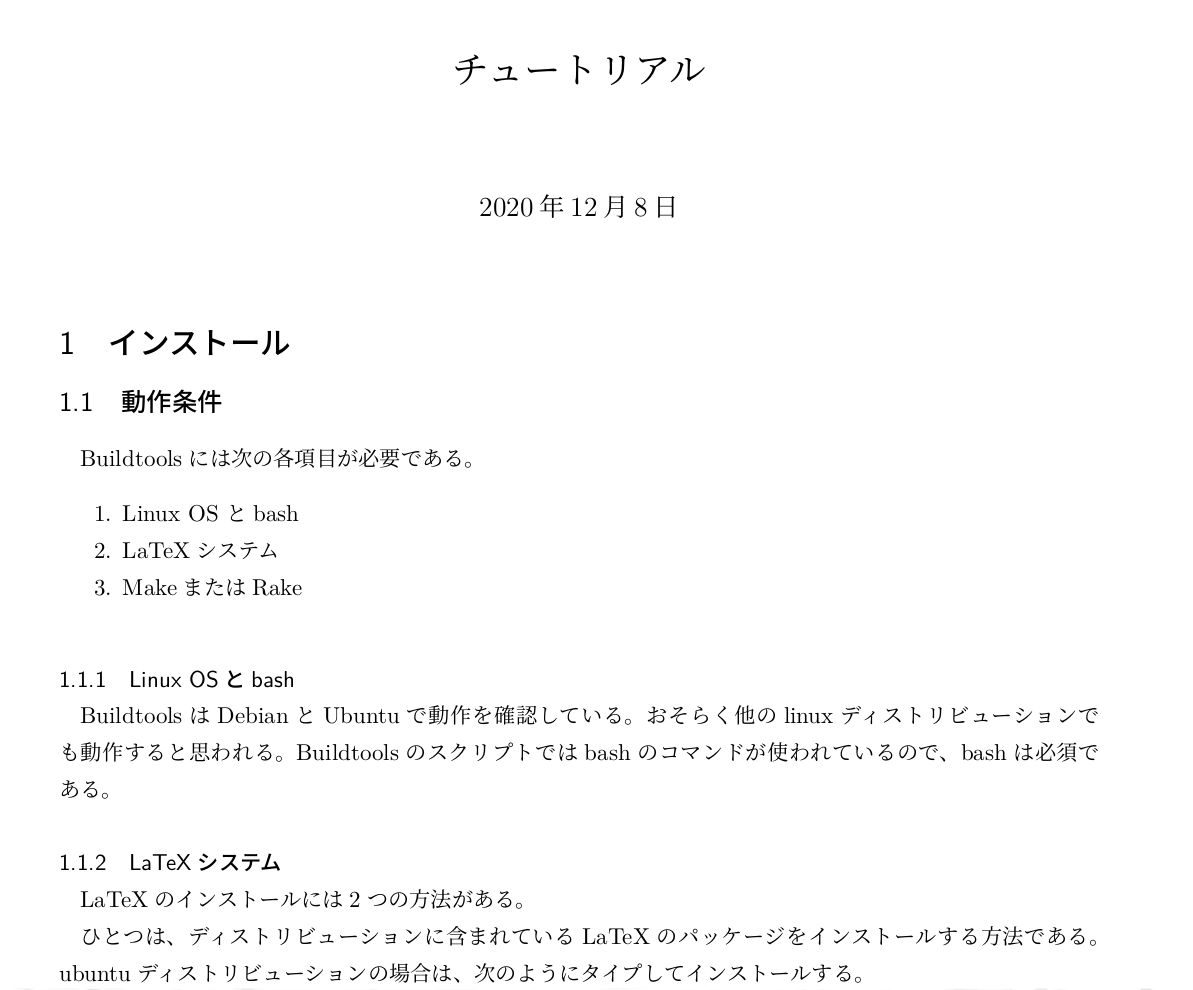
\includegraphics[width=12cm]{Tutorial_2.png}
\end{center}
